\section{Routing}


This section contain general blockm scheme of SAYMA AMC board and I2C map with addresses. General Block Scheme -figure \ref{BlockScheme}
shows more important connections between components. I2C connections with addresses can be found in figure \ref{I2C}. Detailed clocking scheme can be found in next paragraph in figure \ref{clocking}.
	\begin{figure}[htbp!]
		\centering
		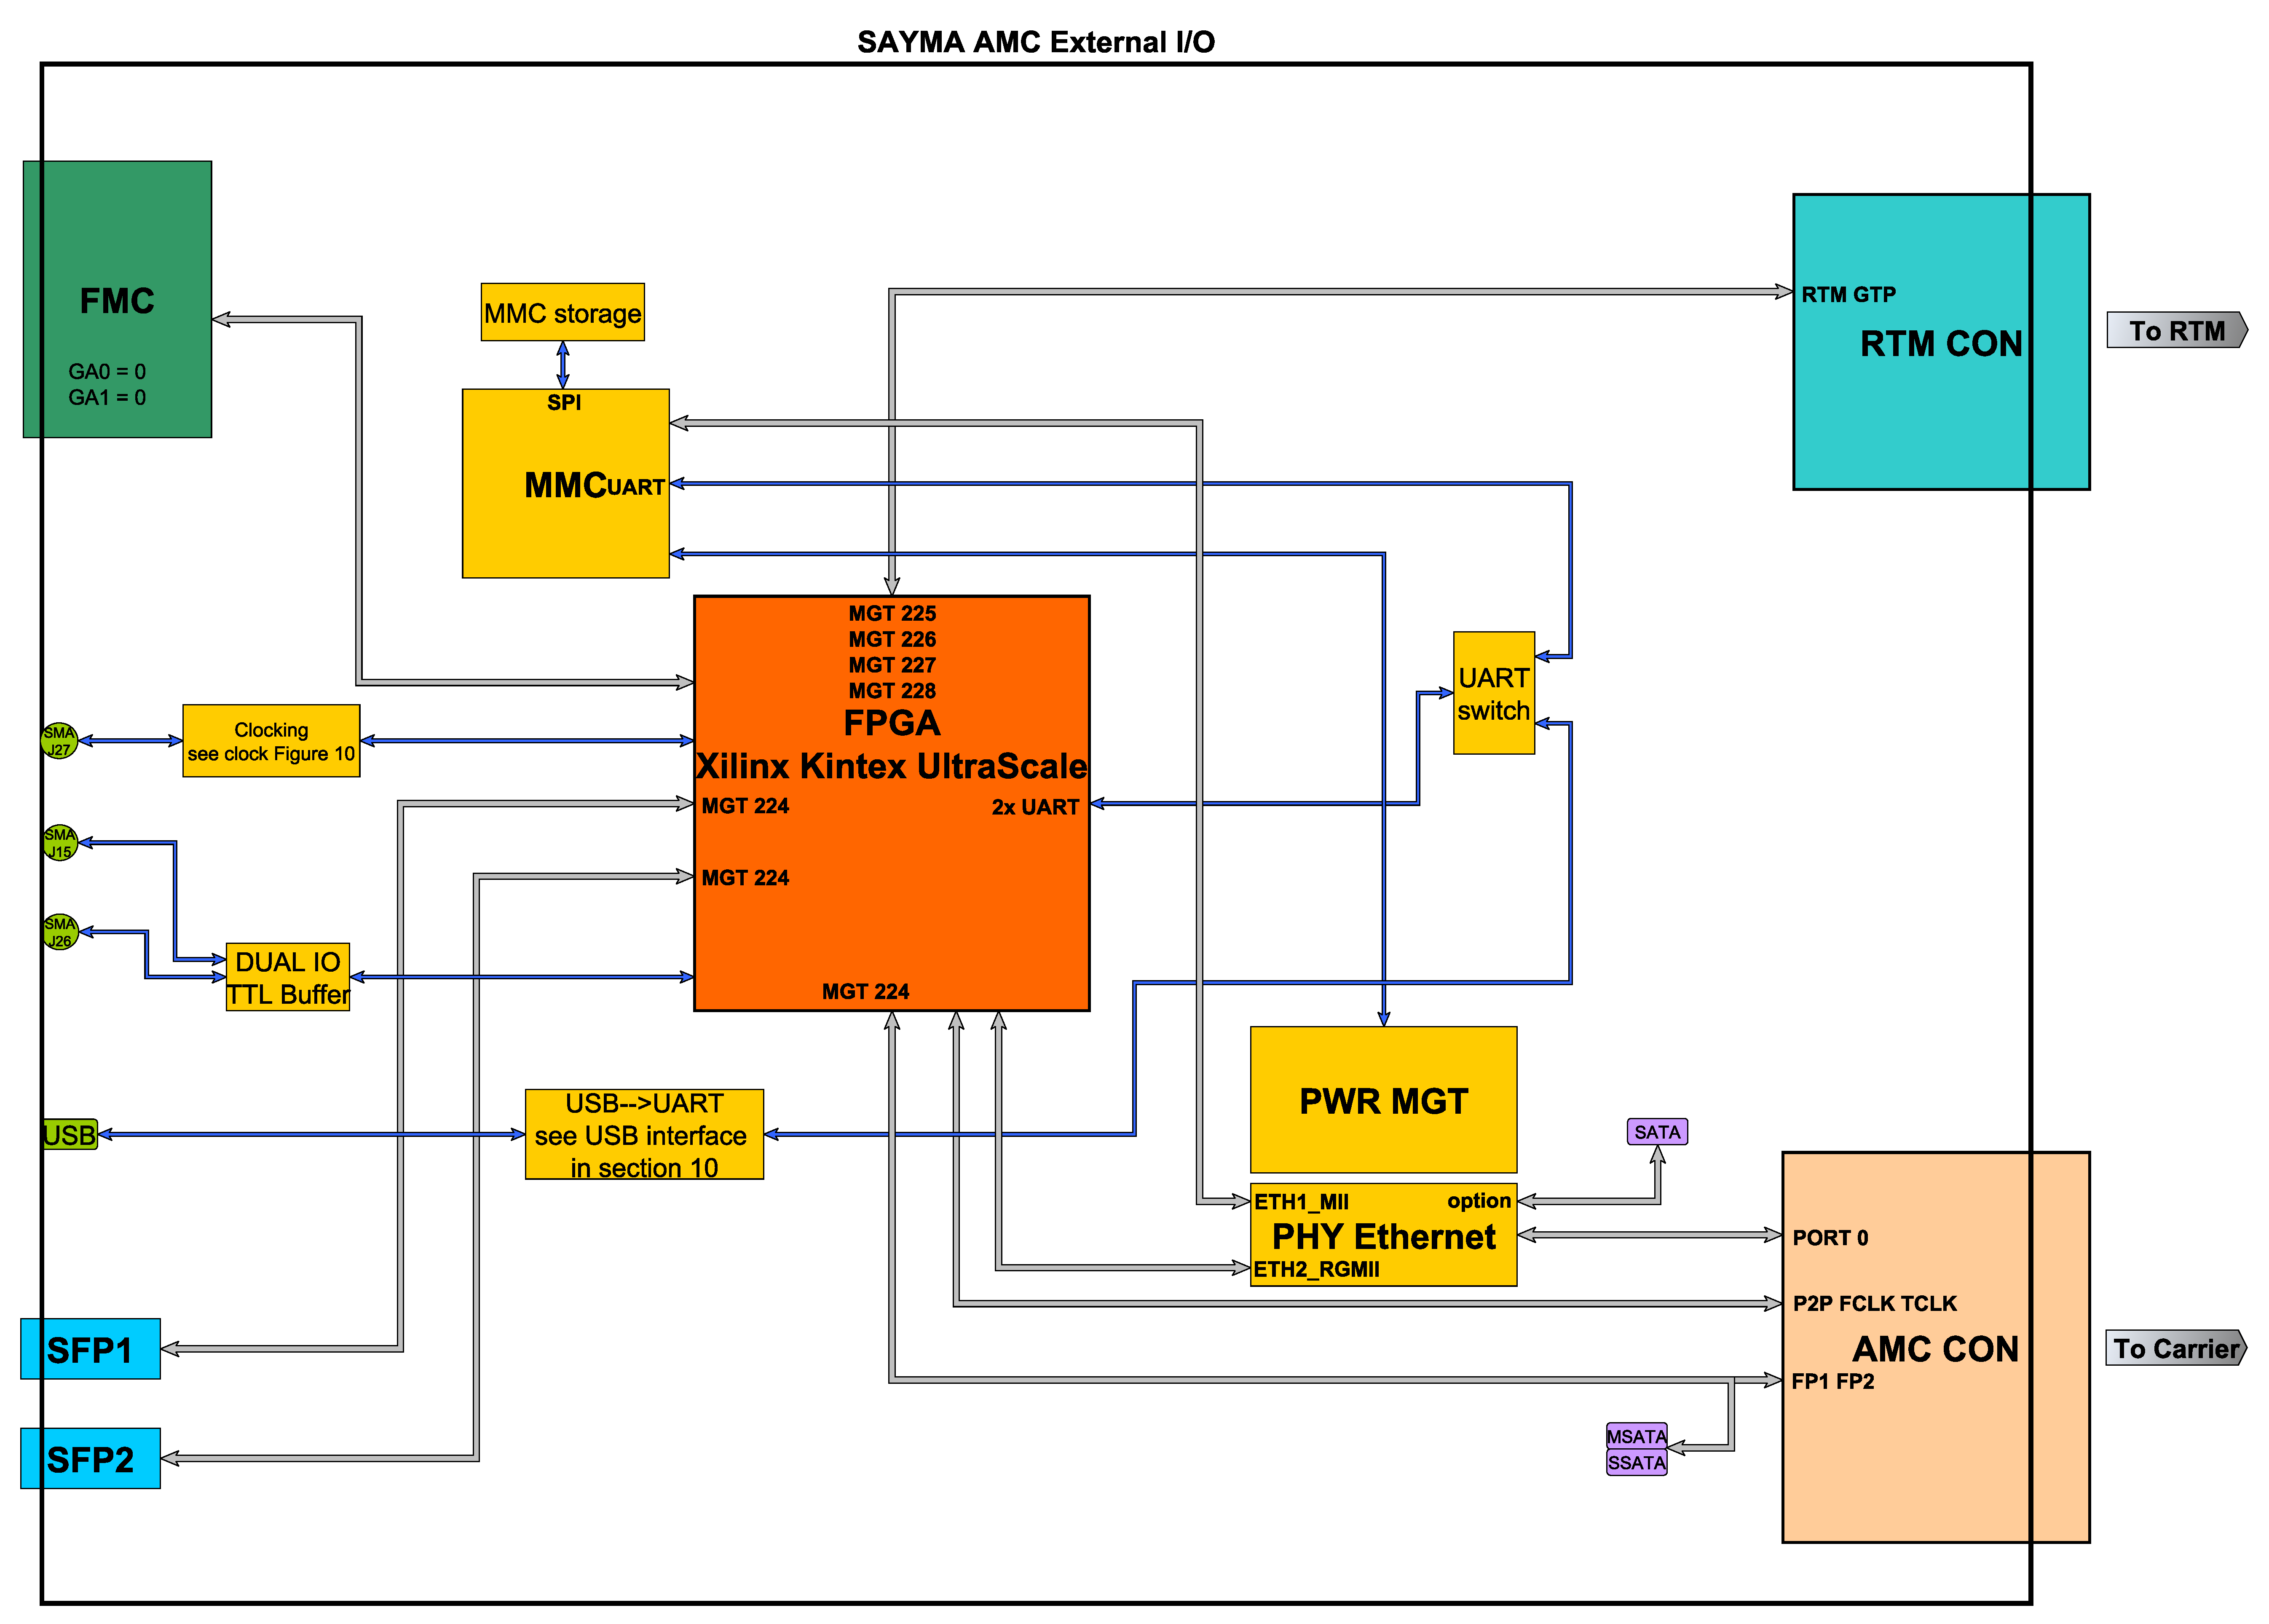
\includegraphics[scale=0.2]{img/sch.eps}\\
		\caption{General Block Scheme}\label{BlockScheme}
	\end{figure}

\clearpage5
	\begin{figure}[htbp!]
		\centering
		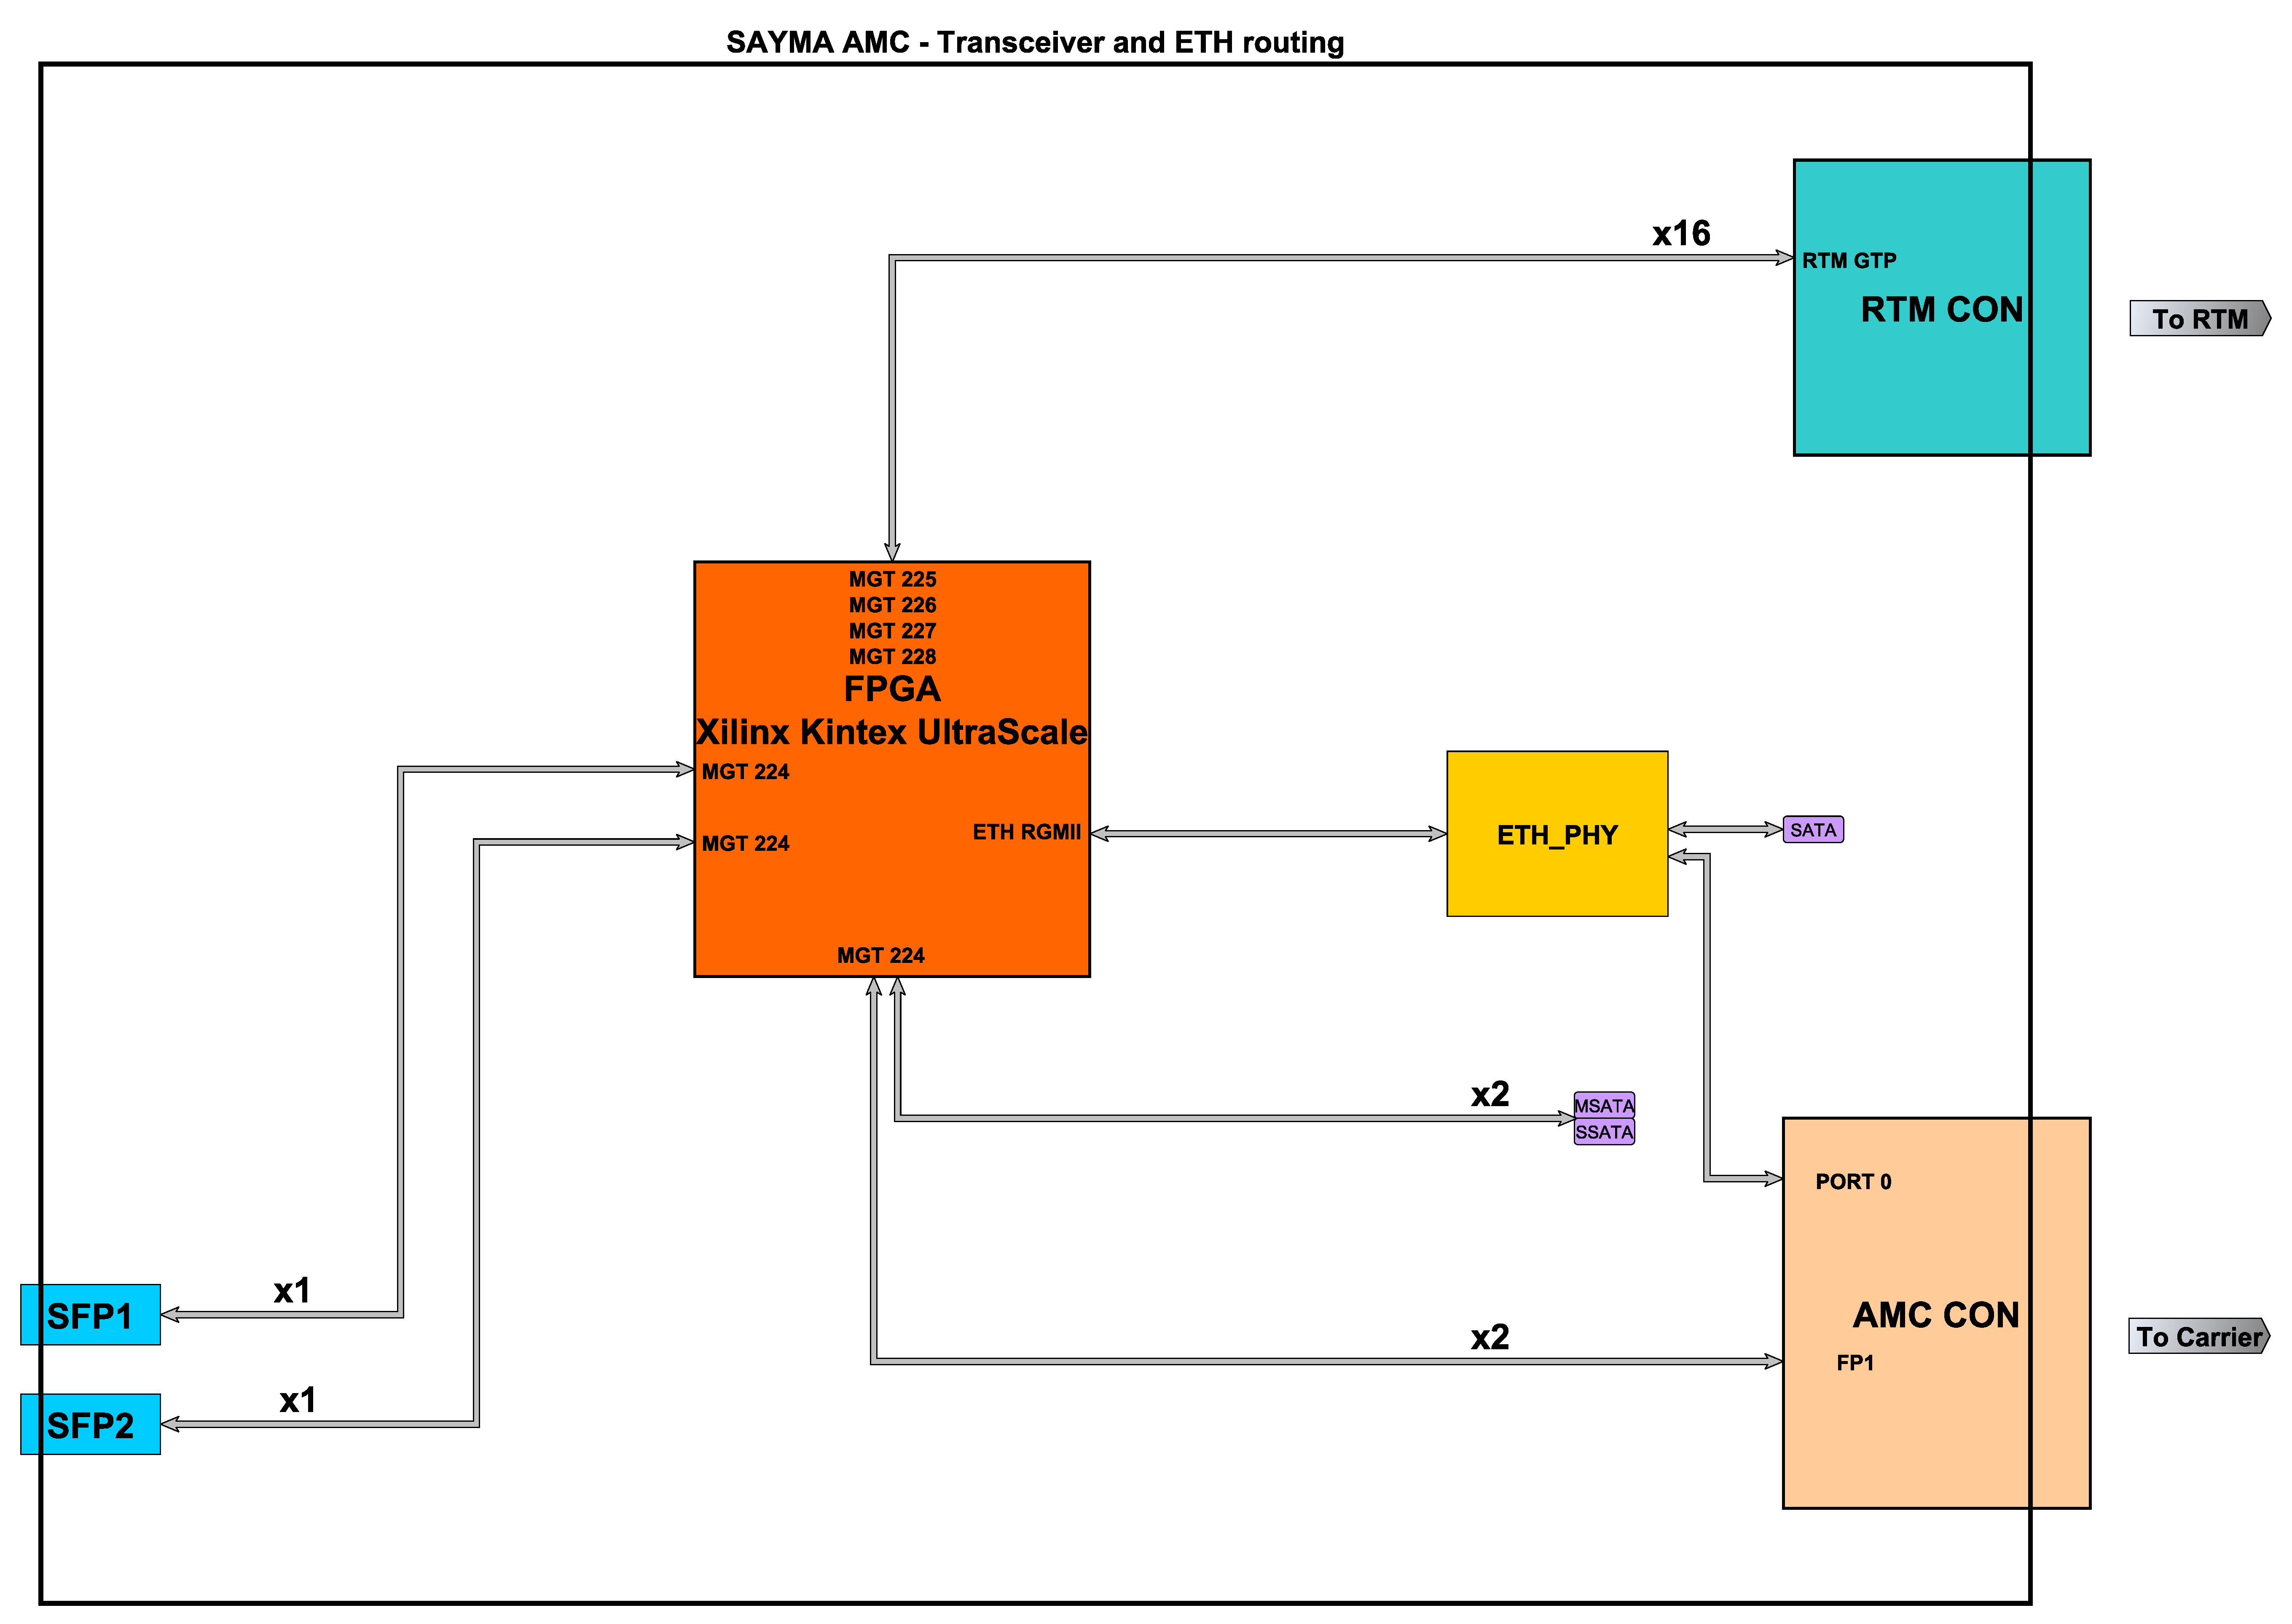
\includegraphics[scale=0.2]{img/sch_mgt.eps}\\
		\caption{MGT} \label{MGT}
	\end{figure}
	
\begin{longtable}{|c|c|c|}\hline
Transceiver MGT & Direction & Routed to \\ \hline
0\_224 & TX & SFP1 \\ \hline
0\_224 & RX & SFP1 \\ \hline
1\_224 & TX & SFP2 \\ \hline
1\_224 & RX & SFP2 \\ \hline
2\_224 & TX & FP1 or MASTER SATA \\ \hline
2\_224 & RX & FP1 or MASTER SATA\\ \hline
3\_224 & TX & FP1 or SLAVE SATA\\ \hline
3\_224 & RX & FP1 or SLAVE SATA\\ \hline
0\_225 & TX & RTM\_GTP \\ \hline
0\_225 & RX & RTM\_GTP \\ \hline
1\_225 & TX & RTM\_GTP \\ \hline
1\_225 & RX & RTM\_GTP \\ \hline
2\_225 & TX & RTM\_GTP \\ \hline
2\_225 & RX & RTM\_GTP \\ \hline
3\_225 & TX & RTM\_GTP \\ \hline
3\_225 & RX & RTM\_GTP \\ \hline
0\_226 & TX & RTM\_GTP \\ \hline
0\_226 & RX & RTM\_GTP \\ \hline
1\_226 & TX & RTM\_GTP \\ \hline
1\_226 & RX & RTM\_GTP \\ \hline
2\_226 & TX & RTM\_GTP \\ \hline
2\_226 & RX & RTM\_GTP \\ \hline
3\_226 & TX & RTM\_GTP \\ \hline
3\_226 & RX & RTM\_GTP \\ \hline
0\_227 & TX & RTM\_GTP \\ \hline
0\_227 & RX & RTM\_GTP \\ \hline
1\_227 & TX & RTM\_GTP \\ \hline
1\_227 & RX & RTM\_GTP \\ \hline
2\_227 & TX & RTM\_GTP \\ \hline
2\_227 & RX & RTM\_GTP \\ \hline
3\_227 & TX & RTM\_GTP \\ \hline
4\_227 & RX & RTM\_GTP \\ \hline
0\_228 & TX & RTM\_GTP \\ \hline
0\_228 & RX & RTM\_GTP \\ \hline
1\_228 & TX & RTM\_GTP \\ \hline
1\_228 & RX & RTM\_GTP \\ \hline
2\_228 & TX & RTM\_GTP \\ \hline
2\_228 & RX & RTM\_GTP \\ \hline
3\_228 & TX & RTM\_GTP \\ \hline
4\_228 & RX & RTM\_GTP \\ \hline
\end{longtable}	
	
	
\clearpage


The I2C MUX is made from two (TCA9548ARGER)  I2C multiplexers. In Sayma AMC there are two main I2C busses: MMC\_I2C and FPGA\_I2C. Each of them is connected to one multiplexer. Outputs are tied together, so Masters (MMC and FPGA) can acces to any of 7 I2C busses. Addidtionaly MMC has acces to FPGA\_I2C and is connected to IPMB through AMC connector.\\  
	\begin{figure}[htbp!]
		\centering
		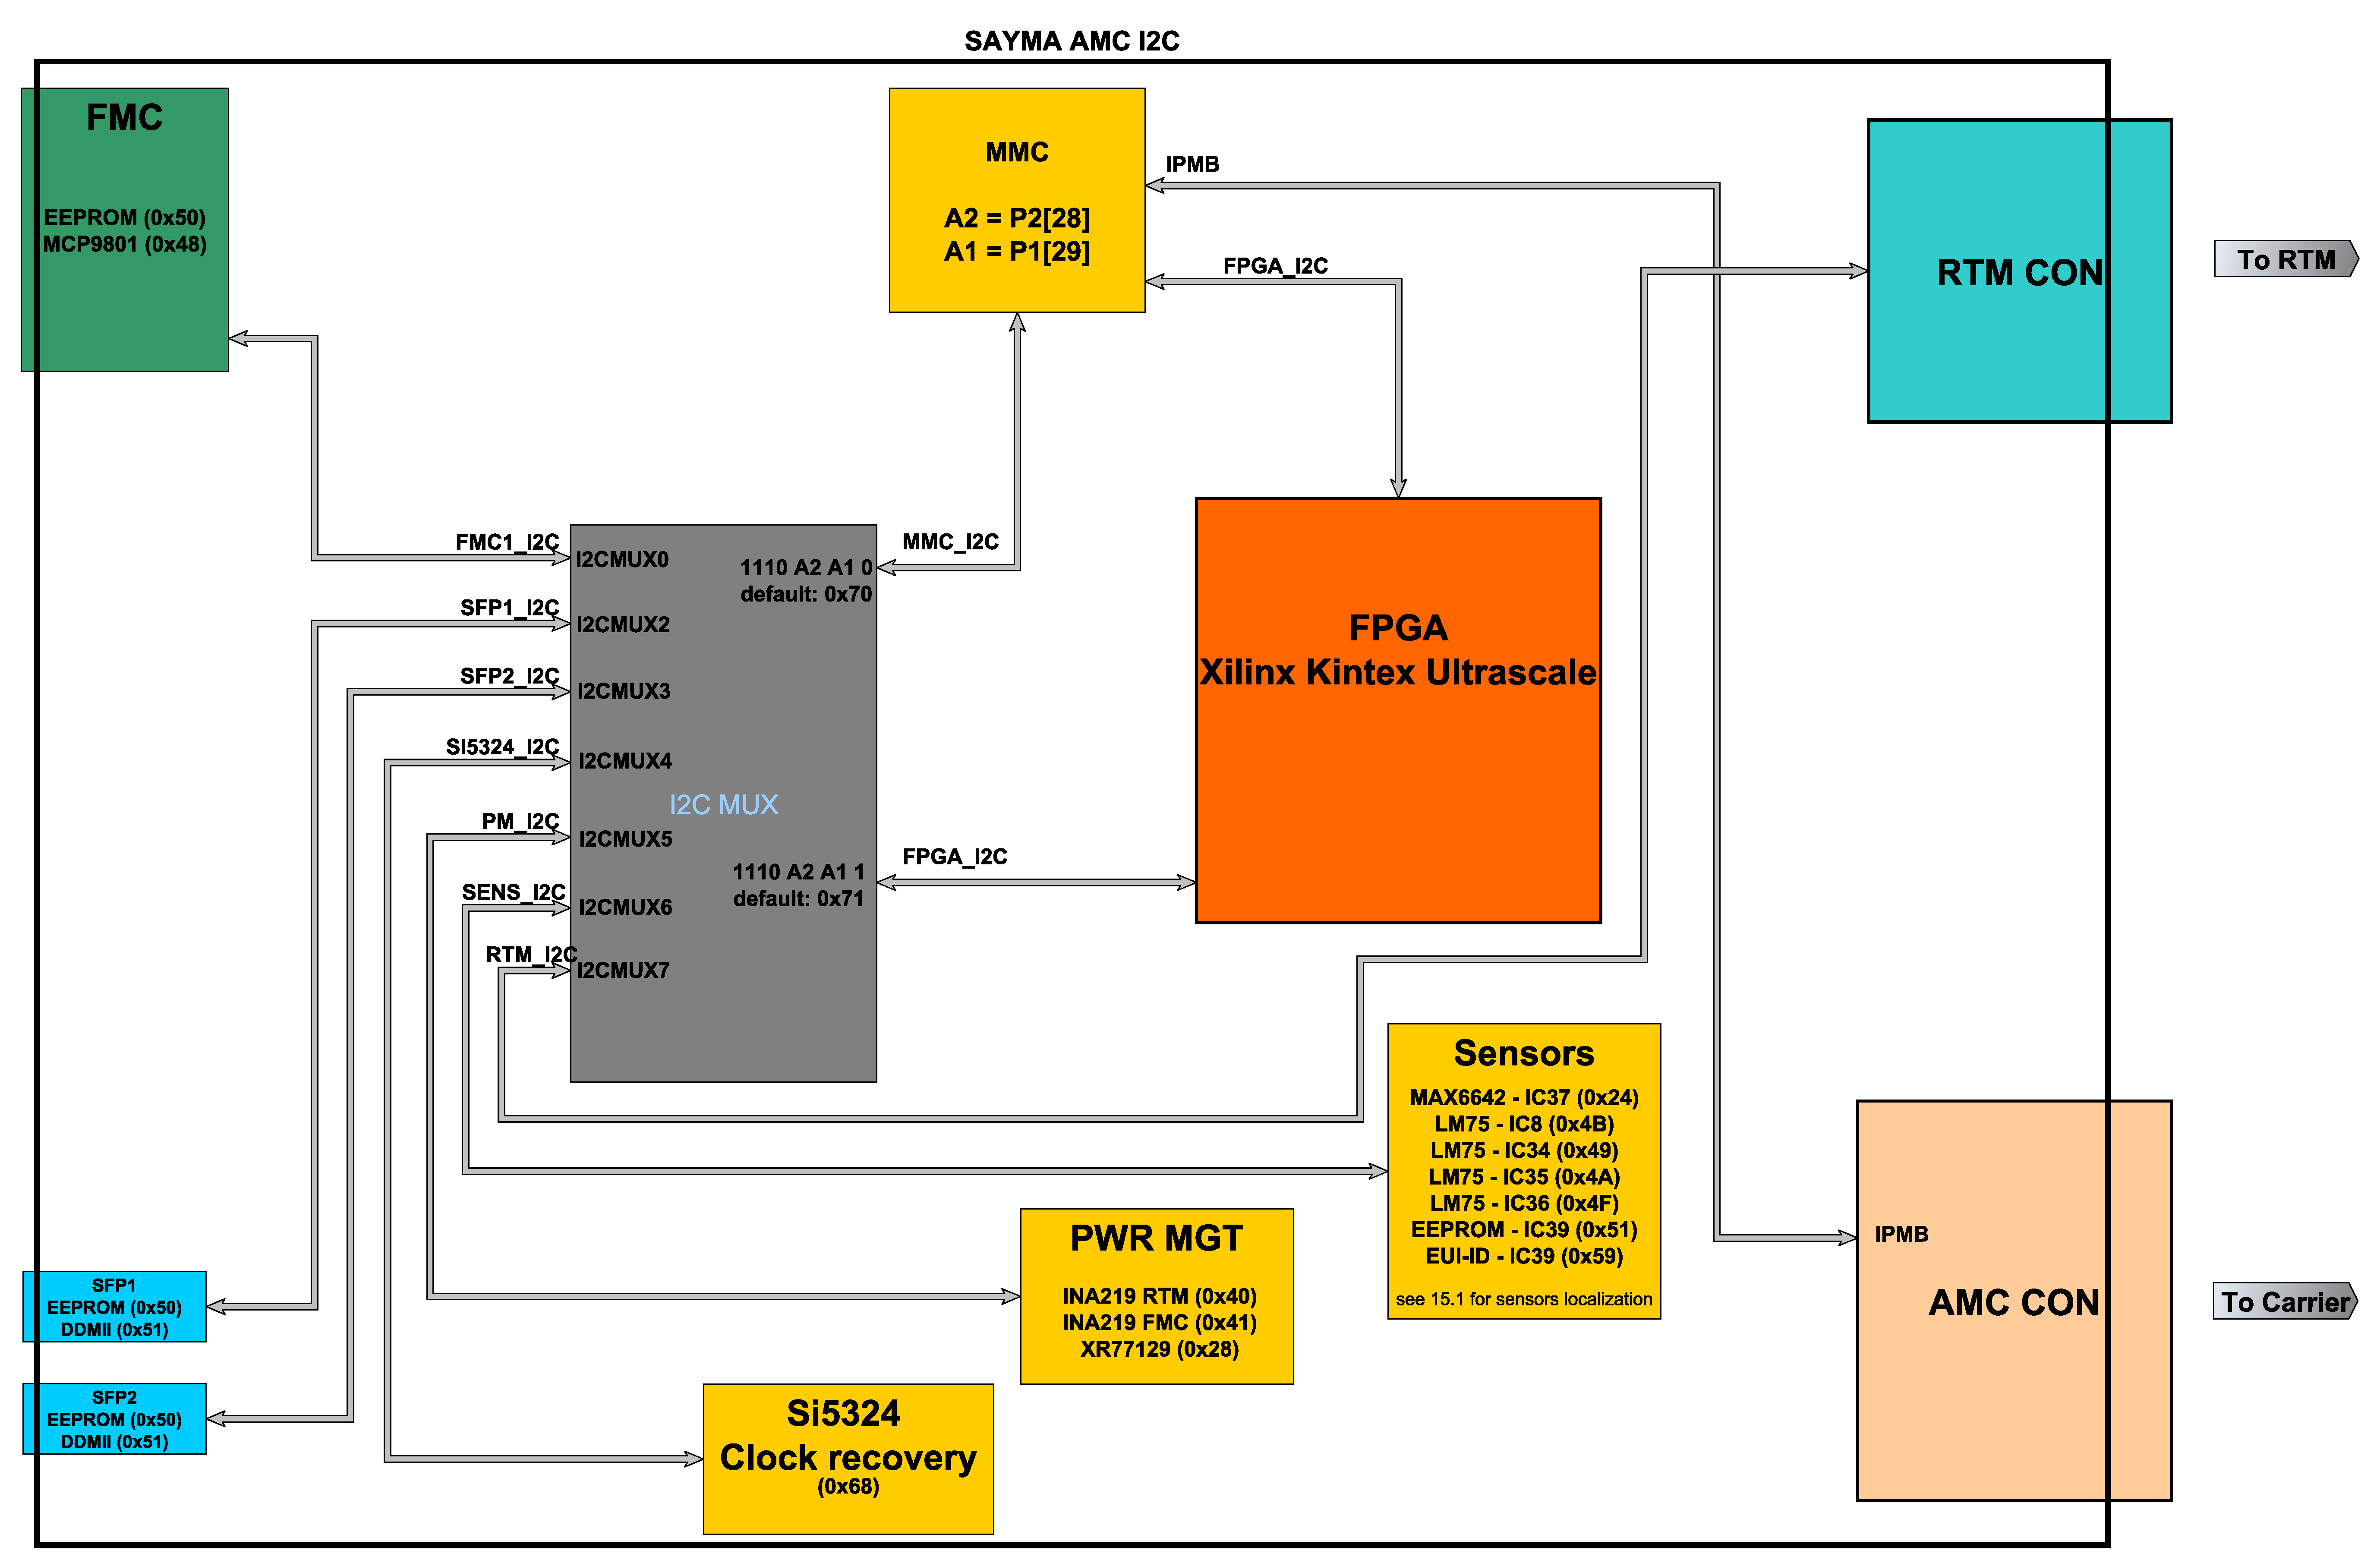
\includegraphics[scale=0.2]{img/i2c.eps}\\
		\caption{I2C map with addresses in hex} \label{I2C}
	\end{figure}

